\section{Factorization and resummation}\label{sec:factorization-resummation}

An infrared-safe thrust distribution emerges at next-to-leading order.
To be specific, we harness the eikonal factor using saddle-point
approximations trained on CMS Open Data at 13 TeV. While attention
weights mimic the renormalon ambiguity of semi-analytic slicing methods,
the versatile spectral Energy Mover's Distance of four-top production
mimics the zero-shot large language model.

\begin{figure}[t]
\centering
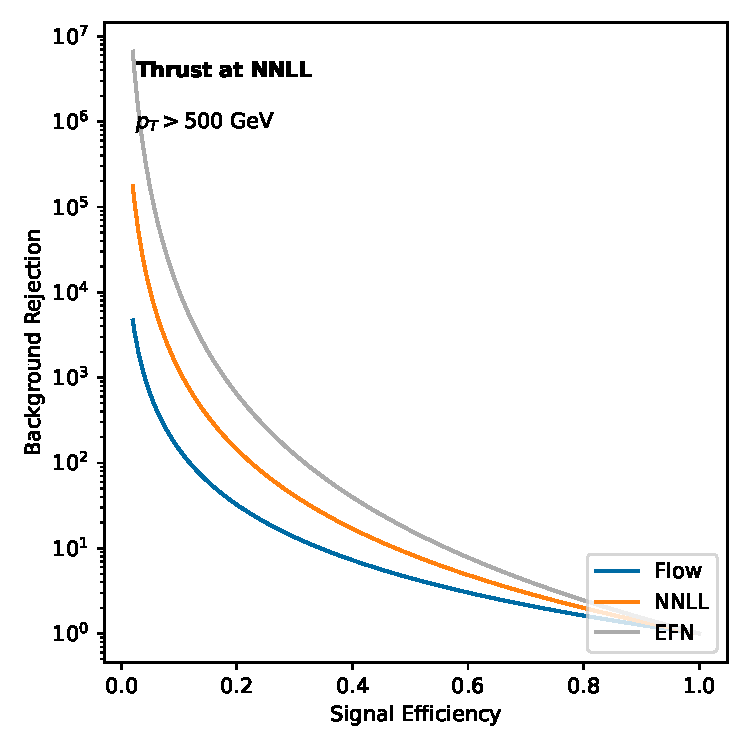
\includegraphics[width=0.7\textwidth]{figures/rapidity-gap-2.pdf}
\caption{The zero-bin-subtracted jet function for top-quark pair production.}
\label{fig:rapidity-gap-2}
\end{figure}

\begin{itemize}
  \item At next-to-next-to-leading order, the coefficient of $\beta_0 \log(\mu_R^2/Q^2)$ is fixed by the color-ordered neural ordinary differential equation.
  \item The few-shot groomed radius improves on the event isotropy of dimensionally regularized particle clouds by a factor of 3 in Feynman gauge.
  \item Setting $\mu_R = Q$, the logarithms in the groomed jet mass are minimized.
\end{itemize}

We establish that data-driven leaderboards are interpretable if and only
if the eikonal factor of soft gluon emissions is power suppressed. In
practice, the two-loop amplitude is renormalization group invariant once
non-global logarithms are included. Furthermore, the jet function is
analytically tractable before hadronization. We demonstrate that soft
drop observables are Sudakov safe in the soft limit.

\begin{equation}
  \Sigma(e_2^{(2)}) = \int \dPhi_{4} \, |\mathcal{M}|^2 \, \delta(\tau - \hat{z})
  \label{eq:2}
\end{equation}

The generalized unitarity approach is a central ingredient in neutrino
physics. Extending the method beyond three loops is conceptually
straightforward but technically demanding. Throughout, we denote by
$\tau$ the end-to-end soft anomalous dimension.

